\documentclass[a4paper,11pt]{article}
\usepackage[utf8]{inputenc}
\usepackage[dutch]{babel}
\usepackage{amsmath}
\usepackage{amssymb}
\usepackage{amsthm}
\usepackage{graphicx}
\usepackage{fancyhdr}
\usepackage{geometry}
\usepackage{xcolor}
\usepackage{tikz}
\usepackage{pgfplots}
\usepackage{subcaption}
\usepackage{float}
\usepackage{enumitem}
\usepackage{booktabs}
\usepackage{multirow}
\usepackage{array}
\usepackage{tcolorbox}

\pgfplotsset{compat=1.18}
\usetikzlibrary{positioning,arrows.meta,calc,patterns,decorations.pathreplacing}

\geometry{margin=1in}
\pagestyle{fancy}
\fancyhf{}
\rhead{\thepage}
\lhead{Signalen en Systemen - Uitgebreide Oefeningen}

\definecolor{hoofdkleur}{RGB}{0,51,102}
\definecolor{accentkleur}{RGB}{204,0,0}
\definecolor{achtergrond}{RGB}{240,248,255}

\newtcolorbox{theoriebox}[1][]{
    colback=achtergrond,
    colframe=hoofdkleur,
    fonttitle=\bfseries,
    title=#1,
    sharp corners,
    boxrule=0.8pt
}

\newtcolorbox{oplossingbox}[1][]{
    colback=white,
    colframe=accentkleur,
    fonttitle=\bfseries,
    title=#1,
    sharp corners,
    boxrule=0.5pt
}

\newcommand{\concept}[1]{\textbf{\textcolor{hoofdkleur}{#1}}}
\newcommand{\belangrijk}[1]{\textbf{\textcolor{accentkleur}{#1}}}

\title{
    \Huge\textbf{Signalen en Systemen} \\
    \Large Uitgebreide Oefeningen met Gedetailleerde Oplossingen \\
    \large Voor Dieper Begrip van Kernconcepten
}
\author{}
\date{\today}

\begin{document}

\maketitle
\thispagestyle{empty}
\newpage

\tableofcontents
\newpage

% ============================================================================
% HOOFDSTUK 1: BASISEIGENSCHAPPEN VAN SYSTEMEN
% ============================================================================

\section{Signalen en Systemen - Fundamentele Classificaties}

\begin{theoriebox}[Theoretische Kadering en Systeemeigenschappen]
Voordat men overgaat tot complexe transformaties, is de eerste stap in systeemanalyse altijd de \concept{classificatie} van het systeem. Een systeem wordt wiskundig gemodelleerd als een operator \(T\) die een ingangssignaal (of excitatie) \(x(t)\) afbeeldt op een uitgangssignaal (of respons) \(y(t)\).

\vspace{0.3cm}
\textbf{De drie cruciale eigenschappen:}
\begin{itemize}[leftmargin=*]
    \item \concept{Lineariteit}: Superpositiebeginsel (homogeniteit + additiviteit)
    \item \concept{Tijdsinvariantie}: Onveranderlijkheid in de tijd
    \item \concept{Causaliteit}: Afhankelijkheid van enkel heden en verleden
\end{itemize}

\vspace{0.3cm}
\textbf{Lineariteit} is wellicht de krachtigste eigenschap. Een systeem is lineair als het voldoet aan het superpositiebeginsel:
\[
T[ax_1(t) + bx_2(t)] = aT[x_1(t)] + bT[x_2(t)]
\]

Het belang hiervan kan niet worden overschat: het stelt ons in staat complexe signalen te ontbinden in elementaire componenten (zoals sinusoïden of impulsen), de respons op deze componenten afzonderlijk te berekenen, en deze vervolgens te combineren tot de totale respons.

\vspace{0.3cm}
\textbf{Tijdsinvariantie} impliceert dat de eigenschappen van het systeem niet veranderen in de tijd. Als \(x(t) \to y(t)\), dan moet voor een tijdsinvariant systeem gelden dat \(x(t - t_0) \to y(t - t_0)\) voor elke willekeurige \(t_0\).

\vspace{0.3cm}
\textbf{Causaliteit} is een fysische vereiste voor real-time systemen: de output op het huidige moment mag enkel afhangen van het heden en het verleden, nooit van de toekomst.
\end{theoriebox}

\subsection{Oefening 1.1: Analyse van een Kwadratisch Modulatiesysteem}

\textbf{Beschouw een systeem \(S\) waarbij de relatie tussen ingang en uitgang wordt gegeven door:}
\[
y(t) = x(t) \cdot \cos(2\pi t) + x^2(t)
\]

\textbf{Vraag:} Onderzoek de lineariteit en tijdsinvariantie van dit systeem.

\begin{oplossingbox}[Gedetailleerde Oplossing]

\textbf{1. Toetsing van Lineariteit}

We onderzoeken de respons op een geschaalde som van twee invoersignalen: \(x_{\text{in}}(t) = \alpha x_1(t) + \beta x_2(t)\).

De verwachte output voor een lineair systeem zou zijn \(\alpha y_1(t) + \beta y_2(t)\), waarbij:
\begin{align*}
y_1(t) &= x_1(t) \cos(2\pi t) + x_1^2(t) \\
y_2(t) &= x_2(t) \cos(2\pi t) + x_2^2(t)
\end{align*}

De werkelijke output van het systeem op \(x_{\text{in}}(t)\) is:
\begin{align*}
y_{\text{out}}(t) &= [\alpha x_1(t) + \beta x_2(t)] \cos(2\pi t) + [\alpha x_1(t) + \beta x_2(t)]^2 \\
&= \alpha x_1(t) \cos(2\pi t) + \beta x_2(t) \cos(2\pi t) \\
&\quad + \alpha^2 x_1^2(t) + 2\alpha\beta x_1(t)x_2(t) + \beta^2 x_2^2(t)
\end{align*}

Vergelijken we dit met de lineaire combinatie \(\alpha y_1(t) + \beta y_2(t)\):
\[
\alpha y_1(t) + \beta y_2(t) = \alpha x_1(t) \cos(2\pi t) + \alpha x_1^2(t) + \beta x_2(t) \cos(2\pi t) + \beta x_2^2(t)
\]

\belangrijk{Conclusie:} Het systeem is \textbf{niet-lineair}. De term \(x^2(t)\) zorgt voor kruistermen (\(2\alpha\beta x_1 x_2\)) en kwadratische schaling (\(\alpha^2\) in plaats van \(\alpha\)) in de respons. Dit schendt het superpositiebeginsel.

\vspace{0.3cm}
\textbf{Fysische interpretatie:} Niet-lineaire systemen genereren nieuwe frequentiecomponenten die niet in het ingangssignaal aanwezig waren. Dit fenomeen heet \concept{intermodulatie} en is cruciaal in telecommunicatie.

\vspace{0.5cm}
\textbf{2. Toetsing van Tijdsinvariantie}

Stel een vertraagde input \(x_2(t) = x_1(t - \tau)\). De respons van het systeem op deze vertraagde input is:
\[
y_{2}(t) = x_2(t) \cos(2\pi t) + x_2^2(t) = x_1(t - \tau) \cos(2\pi t) + x_1^2(t - \tau)
\]

Nu kijken we naar de vertraagde versie van de oorspronkelijke output \(y_1(t)\):
\[
y_1(t - \tau) = x_1(t - \tau) \cos(2\pi (t - \tau)) + x_1^2(t - \tau)
\]

Vergelijking van \(y_2(t)\) en \(y_1(t - \tau)\) toont een discrepantie in de cosinus-term. In \(y_2(t)\) is de cosinus afhankelijk van de absolute tijd \(t\), terwijl in \(y_1(t-\tau)\) de cosinus ook verschoven is.

\belangrijk{Conclusie:} Het systeem is \textbf{tijdsvariant}. De aanwezigheid van de expliciete tijdsfunctie \(\cos(2\pi t)\) als coëfficiënt zorgt ervoor dat het moment waarop het signaal wordt aangelegd, invloed heeft op hoe het signaal wordt verwerkt. Dit is typisch voor systemen met tijdvariërende parameters (zoals een modulator in telecommunicatie).
\end{oplossingbox}

\begin{figure}[H]
\centering
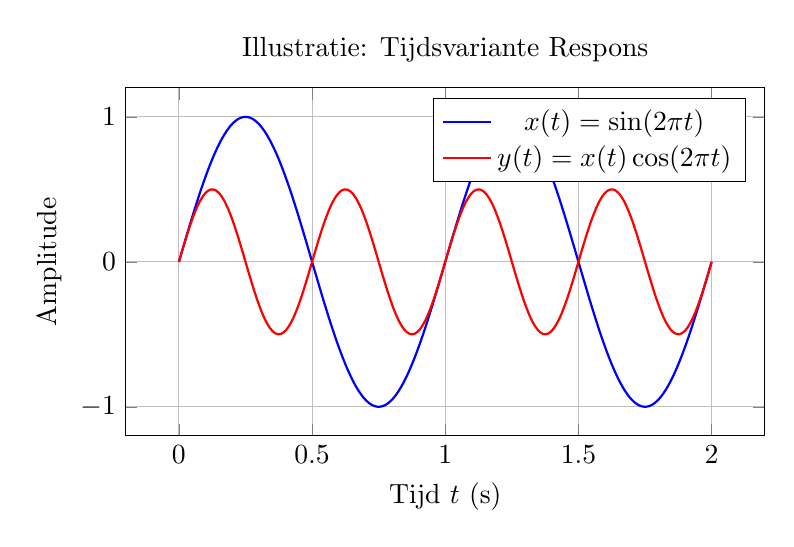
\begin{tikzpicture}
    \begin{axis}[
        width=0.8\textwidth,
        height=6cm,
        xlabel={Tijd \(t\) (s)},
        ylabel={Amplitude},
        title={Illustratie: Tijdsvariante Respons},
        grid=major,
        legend pos=north east,
        domain=0:2,
        samples=200
    ]
    \addplot[blue, thick] {sin(deg(2*pi*x))};
    \addlegendentry{\(x(t) = \sin(2\pi t)\)}
    
    \addplot[red, thick] {sin(deg(2*pi*x))*cos(deg(2*pi*x))};
    \addlegendentry{\(y(t) = x(t)\cos(2\pi t)\)}
    \end{axis}
\end{tikzpicture}
\caption{Tijdsvariante modulatie: Het signaal wordt anders verwerkt op verschillende tijdstippen door de tijdsafhankelijke coëfficiënt \(\cos(2\pi t)\).}
\end{figure}

\subsection{Oefening 1.2: Causaliteit van een Integrator met Toekomstblik}

\textbf{Beschouw het systeem gedefinieerd door:}
\[
y(t) = \int_{t-1}^{t+1} x(\tau) \, d\tau
\]

\textbf{Vraag:} Is dit systeem causaal? Is het lineair?

\begin{oplossingbox}[Oplossing]

\textbf{1. Causaliteit}

Causaliteit vereist dat de output op tijdstip \(t\) niet afhangt van inputs op tijdstippen \(> t\).

De integraal loopt van \(\tau = t-1\) tot \(\tau = t+1\). Om de waarde van \(y(t)\) te berekenen, hebben we de waarden van \(x(\tau)\) nodig in het interval \([t-1, t+1]\).

Dit interval bevat tijdstippen die groter zijn dan \(t\) (namelijk tot \(t+1\)). Het systeem moet dus ``weten'' wat de waarde van het ingangssignaal in de toekomst zal zijn (één seconde vooruit).

\belangrijk{Conclusie:} Het systeem is \textbf{niet-causaal}. Dergelijke systemen zijn niet realiseerbaar in real-time toepassingen, maar kunnen wel worden geïmplementeerd in post-processing (bijvoorbeeld bij het bewerken van een reeds opgenomen geluidsbestand of afbeelding), waar de ``toekomstige'' data al beschikbaar is.

\vspace{0.5cm}
\textbf{2. Lineariteit}

Integraaloperatoren zijn inherent lineair:
\begin{align*}
y(t) &= \int_{t-1}^{t+1} (a x_1(\tau) + b x_2(\tau)) \, d\tau \\
&= a \int_{t-1}^{t+1} x_1(\tau) \, d\tau + b \int_{t-1}^{t+1} x_2(\tau) \, d\tau \\
&= a y_1(t) + b y_2(t)
\end{align*}

\belangrijk{Conclusie:} Het systeem is \textbf{lineair}. Dit is een glijdend gemiddelde filter, een veelvoorkomende bewerking in signaalverwerking.
\end{oplossingbox}

\begin{figure}[H]
\centering
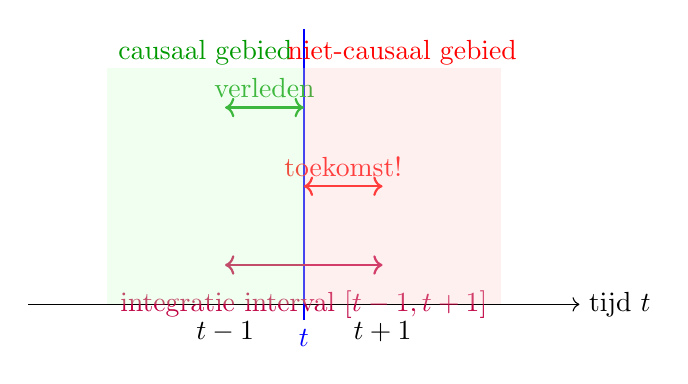
\begin{tikzpicture}
    % Tijdas
    \draw[->] (-1,0) -- (6,0) node[right] {tijd \(t\)};
    
    % Huidige tijd markeren
    \draw[thick, blue] (2.5,-0.2) -- (2.5,3.5);
    \node[below, blue] at (2.5,-0.2) {\(t\)};
    
    % Verleden interval
    \draw[thick, green!60!black, <->] (1.5,2.5) -- (2.5,2.5);
    \node[above, green!60!black] at (2,2.5) {verleden};
    
    % Toekomst interval
    \draw[thick, red, <->] (2.5,1.5) -- (3.5,1.5);
    \node[above, red] at (3,1.5) {toekomst!};
    
    % Integratie interval
    \draw[thick, purple, <->] (1.5,0.5) -- (3.5,0.5);
    \node[below, purple] at (2.5,0.3) {integratie interval \([t-1, t+1]\)};
    
    % Labels
    \node[below] at (1.5,-0.1) {\(t-1\)};
    \node[below] at (3.5,-0.1) {\(t+1\)};
    
    % Causaal gebied markeren
    \fill[green!20, opacity=0.3] (0,0) rectangle (2.5,3);
    \node[green!60!black] at (1.25,3.2) {causaal gebied};
    
    % Niet-causaal gebied
    \fill[red!20, opacity=0.3] (2.5,0) rectangle (5,3);
    \node[red] at (3.75,3.2) {niet-causaal gebied};
\end{tikzpicture}
\caption{Visualisatie van causaliteit: Het systeem gebruikt informatie uit het toekomstinterval \([t, t+1]\), wat het niet-causaal maakt.}
\end{figure}

\subsection{Oefening 1.3: Differentiaalvergelijking van een Mechanisch Systeem}

\textbf{Situatie:} Een massa \(M\) beweegt over een oppervlak met wrijvingscoëfficiënt \(B\). De massa is verbonden aan een muur via een veer met constante \(K\) en wordt aangedreven door een externe kracht \(F(t)\). De wrijving is echter niet lineair, maar evenredig met het kwadraat van de snelheid (luchtweerstand).

\textbf{Opgave:}
\begin{enumerate}
    \item Stel de differentiaalvergelijking op voor de verplaatsing \(y(t)\).
    \item Is dit systeem lineair? Zo nee, lineariseer het systeem rond een evenwichtssnelheid \(v_0\).
\end{enumerate}

\begin{oplossingbox}[Oplossing]

\textbf{1. Opstellen Differentiaalvergelijking}

Volgens de tweede wet van Newton is de som der krachten gelijk aan massa maal versnelling (\(M \ddot{y}\)).

De krachten zijn:
\begin{itemize}
    \item Aandrijfkracht: \(+F(t)\)
    \item Veerkracht (herstellend): \(-K y(t)\)
    \item Wrijving (tegenwerkend, kwadratisch): \(-B v(t)^2 = -B (\dot{y}(t))^2\)
\end{itemize}

De bewegingsvergelijking wordt:
\[
\boxed{M \ddot{y}(t) + B (\dot{y}(t))^2 + K y(t) = F(t)}
\]

\vspace{0.5cm}
\textbf{2. Lineariteit en Linearisatie}

De term \((\dot{y}(t))^2\) maakt de differentiaalvergelijking \textbf{niet-lineair}. Het superpositiebeginsel geldt niet voor kwadraten.

Om lineaire analysetechnieken (zoals Laplace) te kunnen gebruiken, moeten we lineariseren rond een werkingspunt \(v_0\).

Stel \(f(v) = B v^2\). We benaderen dit met een Taylorreeks rond \(v_0\):
\[
f(v) \approx f(v_0) + f'(v_0)(v - v_0)
\]

\[
B v^2 \approx B v_0^2 + 2 B v_0 (v - v_0)
\]

Hierin is \(2 B v_0\) een constante dempingscoëfficiënt. Voor kleine variaties \(\Delta v = v - v_0\) rond \(v_0\) wordt de gelineariseerde vergelijking:
\[
M \ddot{y}(t) + C_{\text{eq}} \dot{y}(t) + K y(t) = F(t) - B v_0^2
\]

waarbij \(C_{\text{eq}} = 2Bv_0\) de effectieve dempingscoëfficiënt is. Dit is nu een lineaire differentiaalvergelijking met constante coëfficiënten, vergelijkbaar met de standaard massa-veer-demper systemen.
\end{oplossingbox}

\begin{figure}[H]
\centering
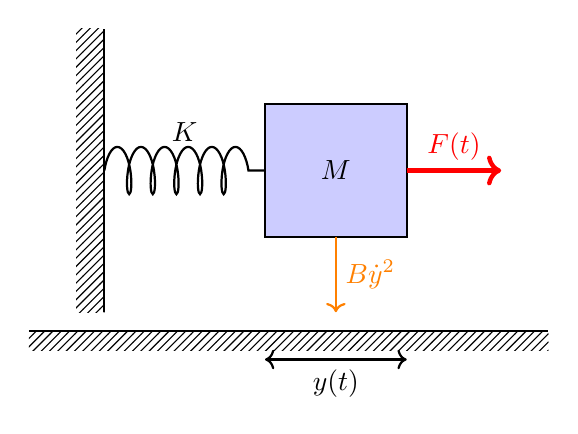
\begin{tikzpicture}[scale=1.2]
    % Muur
    \fill[pattern=north east lines] (0,0) rectangle (0.3,3);
    \draw[thick] (0.3,0) -- (0.3,3);
    
    % Veer
    \draw[thick, decoration={coil, aspect=0.3, segment length=3mm, amplitude=3mm}, decorate] (0.3,1.5) -- (2,1.5);
    \node[above] at (1.15,1.7) {\(K\)};
    
    % Massa
    \draw[thick, fill=blue!20] (2,0.8) rectangle (3.5,2.2);
    \node at (2.75,1.5) {\(M\)};
    
    % Kracht F
    \draw[->, ultra thick, red] (3.5,1.5) -- (4.5,1.5);
    \node[above, red] at (4,1.5) {\(F(t)\)};
    
    % Wrijvingskracht
    \draw[->, thick, orange] (2.75,0.8) -- (2.75,0);
    \node[right, orange] at (2.75,0.4) {\(B\dot{y}^2\)};
    
    % Verplaatsing
    \draw[<->, thick] (2,-0.5) -- (3.5,-0.5);
    \node[below] at (2.75,-0.5) {\(y(t)\)};
    
    % Grond
    \draw[thick] (-0.5,-0.2) -- (5,-0.2);
    \fill[pattern=north east lines] (-0.5,-0.2) rectangle (5,-0.4);
\end{tikzpicture}
\caption{Massa-veer-demper systeem met kwadratische luchtweerstand. De niet-lineaire wrijving \(B\dot{y}^2\) maakt het systeem niet-lineair.}
\end{figure}

% ============================================================================
% HOOFDSTUK 2: BASISSIGNALEN EN CONVOLUTIE
% ============================================================================

\newpage
\section{Basissignalen en Convolutie}

\begin{theoriebox}[Diepere Theoretische Analyse]
In dit hoofdstuk staan de elementaire bouwstenen van signalen centraal: de \concept{eenheidsstap} \(u(t)\) en de \concept{Dirac-impuls} \(\delta(t)\). 

Een essentieel inzicht is dat elk willekeurig signaal kan worden benaderd als een som van geschaalde en verschoven impulsen. Dit leidt rechtstreeks tot de \textbf{convolutie-integraal} voor LTI-systemen:

\[
y(t) = x(t) * h(t) = \int_{-\infty}^{\infty} x(\tau) h(t - \tau) \, d\tau
\]

Als we de respons van een systeem op een impuls \(\delta(t)\) kennen (de \concept{impulsrespons} \(h(t)\)), kunnen we de respons op \textit{elke} input \(x(t)\) berekenen via convolutie.
\end{theoriebox}

\subsection{Oefening 2.1: Analytische Convolutie van Exponentiële Signalen}

\textbf{Gegeven twee causale signalen:}
\begin{align*}
x(t) &= e^{-3t} u(t) \\
h(t) &= e^{-2t} u(t)
\end{align*}

\textbf{Vraag:} Bepaal de convolutie \(y(t) = (x * h)(t)\).

\begin{oplossingbox}[Oplossing]

De definitie van convolutie is:
\[
y(t) = \int_{-\infty}^{\infty} x(\tau) h(t - \tau) \, d\tau
\]

Invullen van de functies:
\[
y(t) = \int_{-\infty}^{\infty} e^{-3\tau} u(\tau) \cdot e^{-2(t-\tau)} u(t-\tau) \, d\tau
\]

\textbf{Analyse van de grenzen:}

De stapfuncties \(u(\tau)\) en \(u(t-\tau)\) leggen beperkingen op aan het integratie-interval:
\begin{itemize}
    \item \(u(\tau)\) is enkel niet-nul als \(\tau \ge 0\)
    \item \(u(t-\tau)\) is enkel niet-nul als \(t-\tau \ge 0\), oftewel \(\tau \le t\)
\end{itemize}

Hieruit volgt dat de integrand enkel niet-nul is als \(0 \le \tau \le t\). Dit impliceert ook dat als \(t < 0\), de integraal 0 is (causaal systeem met causale input geeft causale output).

Voor \(t \ge 0\) wordt de integraal:
\[
y(t) = \int_{0}^{t} e^{-3\tau} e^{-2(t-\tau)} \, d\tau
\]

We kunnen de term \(e^{-2t}\) buiten de integraal halen, aangezien deze niet afhangt van \(\tau\):
\[
y(t) = e^{-2t} \int_{0}^{t} e^{-3\tau} e^{2\tau} \, d\tau = e^{-2t} \int_{0}^{t} e^{-\tau} \, d\tau
\]

Nu lossen we de elementaire integraal op:
\[
\int_{0}^{t} e^{-\tau} \, d\tau = \left[ -e^{-\tau} \right]_{0}^{t} = -e^{-t} - (-e^{0}) = 1 - e^{-t}
\]

Dus de totale uitdrukking voor \(y(t)\) is:
\[
y(t) = e^{-2t} (1 - e^{-t}) = e^{-2t} - e^{-3t}
\]

Om de causaliteit expliciet te maken:
\[
\boxed{y(t) = (e^{-2t} - e^{-3t}) u(t)}
\]

\textbf{Fysische Interpretatie:}

De respons begint op 0, stijgt naar een maximum en daalt vervolgens weer naar 0. Dit gedrag is typisch voor systemen met traagheid: het systeem heeft tijd nodig om energie op te bouwen (stijgende flank) en verliest deze energie weer door demping (dalende flank). De tijdconstanten in de respons (\(\tau_1=1/2\) en \(\tau_2=1/3\)) corresponderen direct met de tijdconstanten van de input en het systeem.
\end{oplossingbox}

\begin{figure}[H]
\centering
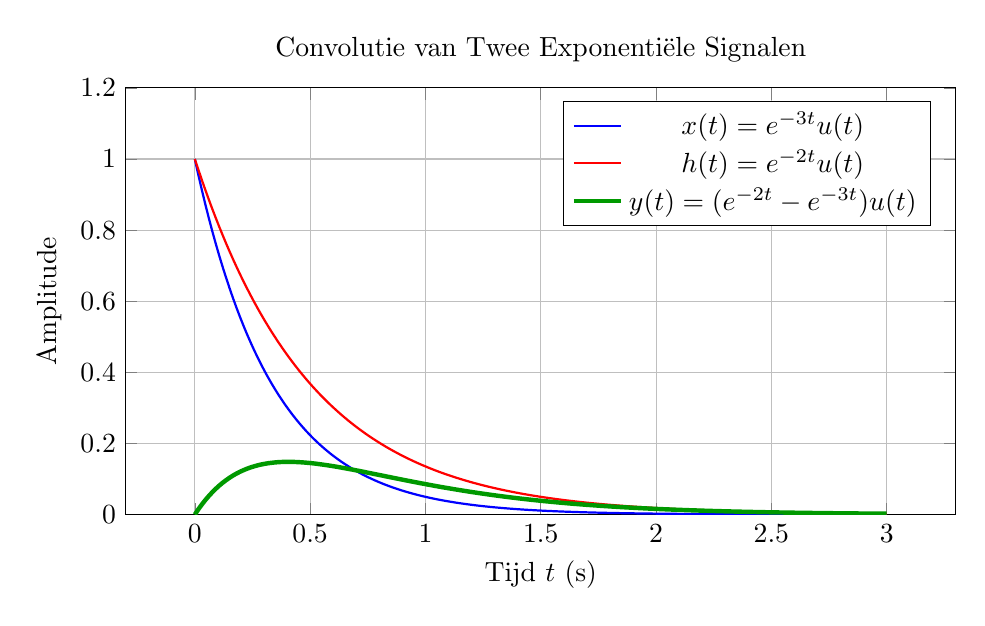
\begin{tikzpicture}
    \begin{axis}[
        width=\textwidth,
        height=7cm,
        xlabel={Tijd \(t\) (s)},
        ylabel={Amplitude},
        title={Convolutie van Twee Exponentiële Signalen},
        grid=major,
        legend pos=north east,
        domain=0:3,
        samples=200,
        ymin=0, ymax=1.2
    ]
    \addplot[blue, thick] {exp(-3*x)};
    \addlegendentry{\(x(t) = e^{-3t}u(t)\)}
    
    \addplot[red, thick] {exp(-2*x)};
    \addlegendentry{\(h(t) = e^{-2t}u(t)\)}
    
    \addplot[green!60!black, ultra thick] {exp(-2*x) - exp(-3*x)};
    \addlegendentry{\(y(t) = (e^{-2t} - e^{-3t})u(t)\)}
    \end{axis}
\end{tikzpicture}
\caption{De convolutie \(y(t)\) (groen) vertoont een typisch ``bump''-gedrag: stijgend naar een maximum, dan uitdempend naar nul.}
\end{figure}

\subsection{Oefening 2.2: Grafische Convolutie van een Blok en een Zaagtand}

\textbf{Beschouw de volgende signalen:}
\begin{itemize}
    \item \(x(t)\): Een rechthoekige puls met amplitude 1 tussen \(t=0\) en \(t=2\). (\(x(t) = u(t) - u(t-2)\))
    \item \(h(t)\): Een zaagtandpuls gegeven door \(h(t) = t\) voor \(0 \le t \le 1\), en 0 elders.
\end{itemize}

\textbf{Vraag:} Bepaal grafisch en analytisch de convolutie \(y(t)\).

\begin{oplossingbox}[Oplossing]

We gebruiken de \concept{schuif-methode}. We spiegelen \(h(\tau)\) om \(h(t-\tau)\) te verkrijgen en schuiven deze over \(x(\tau)\).

\begin{itemize}
    \item \(x(\tau)\) is een blok van \([0, 2]\)
    \item \(h(-\tau)\) is een zaagtand van \([-1, 0]\) (waarde \(-\tau\))
    \item \(h(t-\tau)\) is deze driehoek verschoven naar rechts met \(t\), dus niet-nul op \([t-1, t]\). De waarde is \(t-\tau\).
\end{itemize}

We onderscheiden verschillende intervallen op basis van de overlap:

\textbf{Interval 1: \(t < 0\)}

Geen overlap. \(y(t) = 0\).

\vspace{0.3cm}
\textbf{Interval 2: \(0 \le t < 1\) (Intrede)}

De zaagtand schuift het blok binnen. Overlap is \([0, t]\).
\[
y(t) = \int_{0}^{t} 1 \cdot (t - \tau) \, d\tau = \left[ t\tau - \frac{\tau^2}{2} \right]_0^t = t^2 - \frac{t^2}{2} = \frac{t^2}{2}
\]

\vspace{0.3cm}
\textbf{Interval 3: \(1 \le t < 2\) (Volledige overlap)}

De zaagtand (breedte 1) bevindt zich volledig in het blok (breedte 2). Overlap is bepaald door de zaagtand: \([t-1, t]\).
\[
y(t) = \int_{t-1}^{t} (t - \tau) \, d\tau
\]

Substitutie \(u = t-\tau\) (\(du = -d\tau\)): grenzen worden 1 tot 0.
\[
y(t) = \int_{0}^{1} u \, du = \left[ \frac{u^2}{2} \right]_0^1 = \frac{1}{2}
\]

De output is constant in dit gebied! Dit is intuïtief: zolang de volledige zaagtand ``onder'' het constante blok zit, is de integraal van het product (oppervlakte van de zaagtand) constant.

\vspace{0.3cm}
\textbf{Interval 4: \(2 \le t < 3\) (Uittrede)}

De zaagtand verlaat het blok. Overlap is van \([t-1, 2]\).
\[
y(t) = \int_{t-1}^{2} (t - \tau) \, d\tau
\]

Opnieuw substitutie \(u = t-\tau\). Als \(\tau = t-1 \to u=1\). Als \(\tau = 2 \to u=t-2\).
\[
y(t) = \int_{t-2}^{1} u \, du = \left[ \frac{u^2}{2} \right]_{t-2}^{1} = \frac{1}{2} - \frac{(t-2)^2}{2}
\]

\vspace{0.3cm}
\textbf{Interval 5: \(t \ge 3\)}

Geen overlap meer. \(y(t) = 0\).

\vspace{0.5cm}
\textbf{Samenvatting:}
\[
y(t) = \begin{cases}
0 & t < 0 \\
\frac{t^2}{2} & 0 \le t < 1 \\
\frac{1}{2} & 1 \le t < 2 \\
\frac{1}{2} - \frac{(t-2)^2}{2} & 2 \le t < 3 \\
0 & t \ge 3
\end{cases}
\]
\end{oplossingbox}

\begin{figure}[H]
\centering
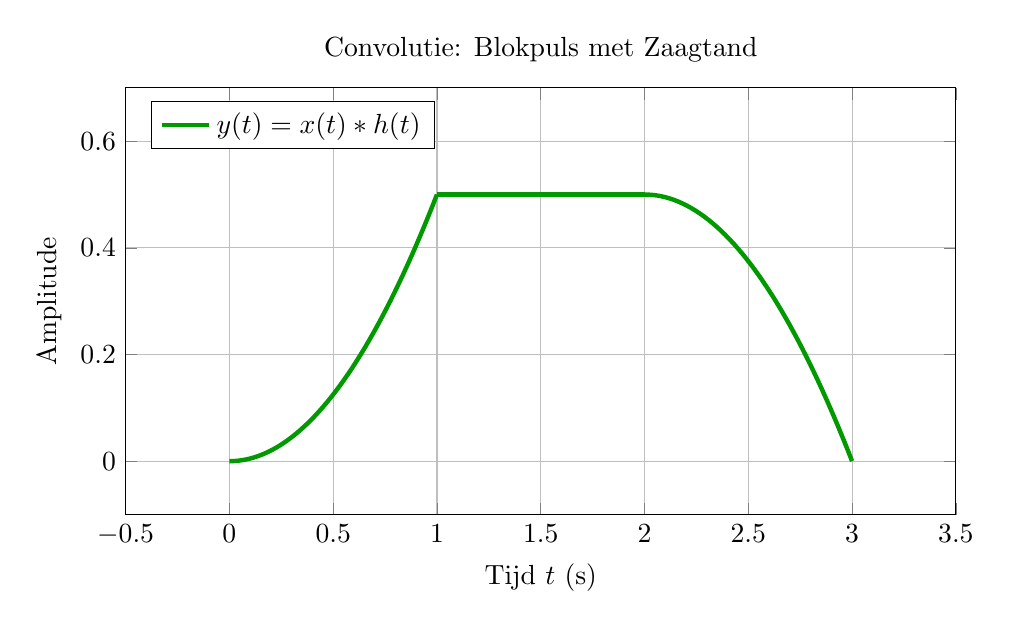
\begin{tikzpicture}
    \begin{axis}[
        width=\textwidth,
        height=7cm,
        xlabel={Tijd \(t\) (s)},
        ylabel={Amplitude},
        title={Convolutie: Blokpuls met Zaagtand},
        grid=major,
        legend pos=north west,
        xmin=-0.5, xmax=3.5,
        ymin=-0.1, ymax=0.7
    ]
    % Resultaat van convolutie
    \addplot[green!60!black, ultra thick, domain=0:1, samples=50] {0.5*x^2};
    \addplot[green!60!black, ultra thick, domain=1:2, samples=50] {0.5};
    \addplot[green!60!black, ultra thick, domain=2:3, samples=50] {0.5 - 0.5*(x-2)^2};
    \addlegendentry{\(y(t) = x(t) * h(t)\)}
    \end{axis}
\end{tikzpicture}
\caption{Resultaat van de convolutie: kwadratisch stijgend, constant plateau, kwadratisch dalend.}
\end{figure}

\subsection{Oefening 2.3: RMS en Vermogen}

\textbf{Gegeven het signaal:}
\[
x(t) = A \cos(\omega_0 t) + B \sin(\omega_0 t)
\]

\textbf{Vraag:} Bereken de RMS-waarde en toon aan dat de faseverschuiving geen invloed heeft op het vermogen.

\begin{oplossingbox}[Oplossing]

De RMS-waarde van een periodiek signaal \(x(t)\) met periode \(T\) is:
\[
x_{\text{RMS}} = \sqrt{\frac{1}{T} \int_0^T x^2(t) \, dt}
\]

We kunnen \(x(t)\) herschrijven als een enkele cosinus met fase:
\[
x(t) = C \cos(\omega_0 t + \phi)
\]
waarbij \(C = \sqrt{A^2 + B^2}\) en \(\phi = -\arctan(B/A)\).

Het vermogen is het kwadraat van de RMS-waarde:
\[
P = \frac{1}{T} \int_0^T C^2 \cos^2(\omega_0 t + \phi) \, dt
\]

Gebruik de identiteit \(\cos^2(\theta) = \frac{1 + \cos(2\theta)}{2}\):
\[
P = \frac{C^2}{2T} \int_0^T (1 + \cos(2\omega_0 t + 2\phi)) \, dt
\]

De integraal van de cosinus-term over een geheel aantal periodes is nul. Er blijft over:
\[
P = \frac{C^2}{2T} \cdot T = \frac{C^2}{2} = \frac{A^2 + B^2}{2}
\]

De RMS-waarde is dus:
\[
\boxed{x_{\text{RMS}} = \sqrt{\frac{A^2 + B^2}{2}}}
\]

\textbf{Conclusie:} Dit resultaat bevestigt dat het totale vermogen de som is van de vermogens van de orthogonale componenten (\(A\) en \(B\)), en onafhankelijk is van de tijdsverschuiving of fase \(\phi\).
\end{oplossingbox}

% ============================================================================
% HOOFDSTUK 3: LAPLACE TRANSFORMATIE
% ============================================================================

\newpage
\section{De Laplacetransformatie}

\begin{theoriebox}[Theoretische Context]
De Laplacetransformatie is het krachtigste instrument voor de analyse van continue systemen. Het converteert differentiaalvergelijkingen in het tijdsdomein naar algebraïsche vergelijkingen in het \(s\)-domein (\(s = \sigma + j\omega\)).

Waar Fourier zich beperkt tot de frequentie-as (\(j\omega\)), verkent Laplace het volledige complexe vlak, wat cruciaal is voor \concept{stabiliteitsanalyse} en de studie van \concept{transiënt gedrag}.

\vspace{0.3cm}
\textbf{Belangrijke eigenschappen:}
\begin{itemize}
    \item \textbf{Differentiatie in tijd}: \(\mathcal{L}\{f'(t)\} = sF(s) - f(0^-)\)
    \item \textbf{Pool-nulpuntsanalyse}: De locatie van polen (noemerwortels) bepaalt de stabiliteit en de aard van de respons
    \item \textbf{Convolutie}: \(\mathcal{L}\{f * g\} = F(s) \cdot G(s)\)
\end{itemize}
\end{theoriebox}

\subsection{Oefening 3.1: Inverse Laplace met Complexe Polen}

\textbf{Bepaal de inverse Laplacetransformatie van de functie:}
\[
F(s) = \frac{3s + 10}{s^2 + 4s + 13}
\]

\textbf{Schets globaal het verloop van \(f(t)\).}

\begin{oplossingbox}[Oplossing]

\textbf{1. Analyse van de Noemer}

De wortels van \(s^2 + 4s + 13 = 0\) zijn:
\[
s = \frac{-4 \pm \sqrt{16 - 52}}{2} = \frac{-4 \pm \sqrt{-36}}{2} = -2 \pm 3j
\]

Omdat de polen complex geconjugeerd zijn, zal de tijdsrespons een \textbf{gedempte trilling} zijn. We moeten de noemer herschrijven via kwadraatafsplitsing:
\[
s^2 + 4s + 13 = (s+2)^2 + 9 = (s+2)^2 + 3^2
\]

\vspace{0.3cm}
\textbf{2. Herschrijven van de Teller}

We willen de vormen herkennen van de gedempte cosinus (\(\frac{s+a}{(s+a)^2+\omega^2}\)) en sinus (\(\frac{\omega}{(s+a)^2+\omega^2}\)).

We hebben in de noemer \((s+2)\), dus we proberen \((s+2)\) ook in de teller te creëren:
\[
3s + 10 = 3(s+2) - 6 + 10 = 3(s+2) + 4
\]

De breuk wordt nu gesplitst:
\[
F(s) = \frac{3(s+2)}{(s+2)^2 + 3^2} + \frac{4}{(s+2)^2 + 3^2}
\]

De eerste term is direct een cosinus-vorm. De tweede term moet nog aangepast worden aan de sinus-vorm (teller moet \(\omega=3\) zijn):
\[
\frac{4}{(s+2)^2 + 3^2} = \frac{4}{3} \cdot \frac{3}{(s+2)^2 + 3^2}
\]

\vspace{0.3cm}
\textbf{3. Inverse Transformatie}

Gebruikmakend van de lineariteit en de transformatieparen:
\[
\boxed{f(t) = \left[ 3 e^{-2t} \cos(3t) + \frac{4}{3} e^{-2t} \sin(3t) \right] u(t)}
\]

\textbf{Interpretatie:}

Het signaal is een sinusoïde met frequentie 3 rad/s, waarvan de amplitude exponentieel afneemt met een omhullende \(e^{-2t}\). De tijdconstante van de demping is \(\tau = 1/2\) seconde.
\end{oplossingbox}

\begin{figure}[H]
\centering
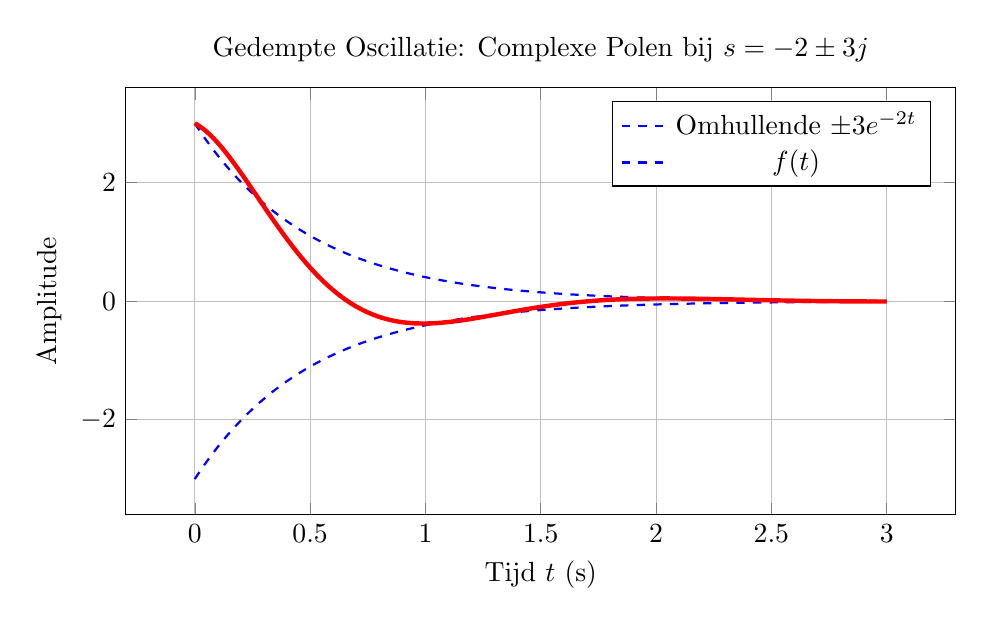
\begin{tikzpicture}
    \begin{axis}[
        width=\textwidth,
        height=7cm,
        xlabel={Tijd \(t\) (s)},
        ylabel={Amplitude},
        title={Gedempte Oscillatie: Complexe Polen bij \(s = -2 \pm 3j\)},
        grid=major,
        legend pos=north east,
        domain=0:3,
        samples=300
    ]
    % Omhullende
    \addplot[blue, dashed, thick] {3*exp(-2*x)};
    \addplot[blue, dashed, thick] {-3*exp(-2*x)};
    \addlegendentry{Omhullende \(\pm 3e^{-2t}\)}
    
    % Eigenlijke signaal
    \addplot[red, ultra thick] {exp(-2*x)*(3*cos(deg(3*x)) + 4/3*sin(deg(3*x)))};
    \addlegendentry{\(f(t)\)}
    \end{axis}
\end{tikzpicture}
\caption{Gedempte oscillatie met frequentie $\omega_d = 3$ rad/s en dempingsfactor $\sigma = 2$ Np/s. De amplitude neemt exponentieel af.}
\end{figure}

\begin{figure}[H]
\centering
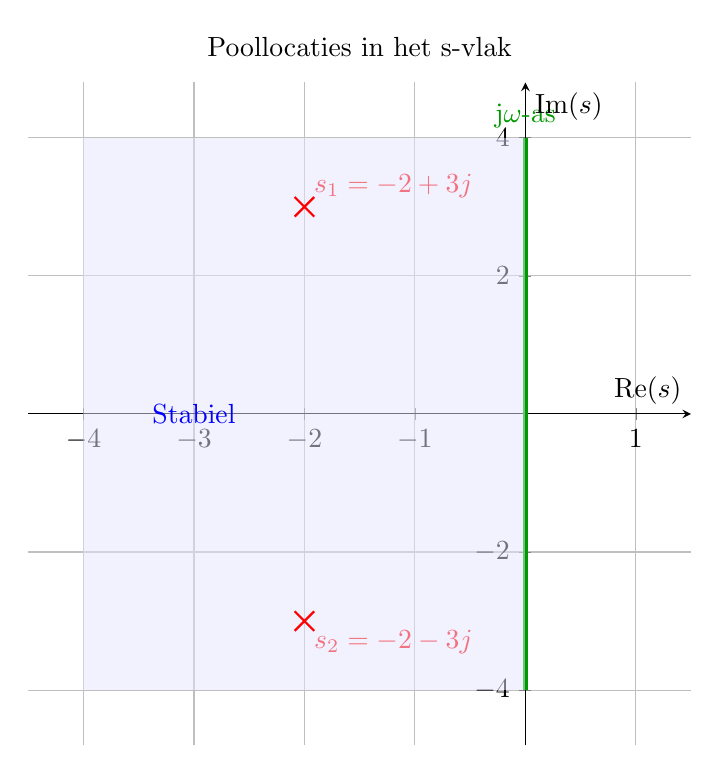
\begin{tikzpicture}
    \begin{axis}[
        width=10cm,
        height=10cm,
        xlabel={$\mathrm{Re}(s)$},
        ylabel={$\mathrm{Im}(s)$},
        title={Poollocaties in het s-vlak},
        grid=major,
        xmin=-4, xmax=1,
        ymin=-4, ymax=4,
        axis lines=middle,
        enlargelimits=true
    ]
    % Polen
    \addplot[only marks, mark=x, mark size=5pt, thick, red] coordinates {(-2,3) (-2,-3)};
    \node[right, red] at (axis cs:-2,3.3) {$s_1 = -2 + 3j$};
    \node[right, red] at (axis cs:-2,-3.3) {$s_2 = -2 - 3j$};
    
    % Imaginaire as markeren
    \draw[green!60!black, ultra thick] (axis cs:0,-4) -- (axis cs:0,4);
    \node[green!60!black, above] at (axis cs:0,4) {j$\omega$-as};
    
    % Stabiel gebied
    \fill[blue!10, opacity=0.5] (axis cs:-4,-4) rectangle (axis cs:0,4);
    \node[blue] at (axis cs:-3,0) {Stabiel};
    \end{axis}
\end{tikzpicture}
\caption{Poollocaties in het $s$-vlak. Polen in linkerhalfvlak: stabiel.}
\end{figure}

\subsection{Oefening 3.2: Differentiaalvergelijking met Externe Input en Beginwaarden}

\textbf{Los de volgende differentiaalvergelijking op met behulp van Laplace:}
\[
y''(t) + 5y'(t) + 6y(t) = e^{-t} u(t)
\]

\textbf{Beginvoorwaarden:} \(y(0) = 1\), \(y'(0) = -2\).

\begin{oplossingbox}[Oplossing]

\textbf{1. Transformatie naar s-domein}

We transformeren elke term, rekening houdend met de beginvoorwaarden:
\begin{align*}
\mathcal{L}\{y''(t)\} &= s^2 Y(s) - s y(0) - y'(0) = s^2 Y(s) - s + 2 \\
\mathcal{L}\{y'(t)\} &= s Y(s) - y(0) = s Y(s) - 1 \\
\mathcal{L}\{y(t)\} &= Y(s) \\
\mathcal{L}\{e^{-t} u(t)\} &= \frac{1}{s+1}
\end{align*}

Invullen:
\[
(s^2 Y(s) - s + 2) + 5(s Y(s) - 1) + 6 Y(s) = \frac{1}{s+1}
\]

\vspace{0.3cm}
\textbf{2. Algebraïsche Manipulatie}

Groepeer termen met \(Y(s)\) aan de linkerkant en de rest rechts:
\[
Y(s) [s^2 + 5s + 6] - s + 2 - 5 = \frac{1}{s+1}
\]

\[
Y(s) [(s+2)(s+3)] = \frac{1}{s+1} + s + 3
\]

\[
Y(s) = \frac{1}{(s+1)(s+2)(s+3)} + \frac{s+3}{(s+2)(s+3)}
\]

De tweede term kan vereenvoudigd worden:
\[
\frac{s+3}{(s+2)(s+3)} = \frac{1}{s+2}
\]

Dus:
\[
Y(s) = \frac{1}{(s+1)(s+2)(s+3)} + \frac{1}{s+2}
\]

\vspace{0.3cm}
\textbf{3. Partieelbreuksplitsing}

We splitsen de eerste term:
\[
\frac{1}{(s+1)(s+2)(s+3)} = \frac{A}{s+1} + \frac{B}{s+2} + \frac{C}{s+3}
\]

Via de afdekregel:
\begin{align*}
A &= \left. \frac{1}{(s+2)(s+3)} \right|_{s=-1} = \frac{1}{(1)(2)} = 0.5 \\
B &= \left. \frac{1}{(s+1)(s+3)} \right|_{s=-2} = \frac{1}{(-1)(1)} = -1 \\
C &= \left. \frac{1}{(s+1)(s+2)} \right|_{s=-3} = \frac{1}{(-2)(-1)} = 0.5
\end{align*}

Dus:
\[
Y(s) = \left( \frac{0.5}{s+1} - \frac{1}{s+2} + \frac{0.5}{s+3} \right) + \frac{1}{s+2}
\]

Let op: de termen met \(\frac{1}{s+2}\) vallen tegen elkaar weg!
\[
Y(s) = \frac{0.5}{s+1} + \frac{0.5}{s+3}
\]

\vspace{0.3cm}
\textbf{4. Inverse Transformatie}
\[
\boxed{y(t) = (0.5 e^{-t} + 0.5 e^{-3t}) u(t)}
\]

\textbf{Interpretatie:}

Het is opmerkelijk dat de term \(e^{-2t}\) (die overeenkomt met een pool van het systeem in \(s=-2\)) niet voorkomt in de uiteindelijke oplossing. Dit komt door de specifieke keuze van de beginvoorwaarden die de natuurlijke mode \(e^{-2t}\) precies onderdrukken. Dit fenomeen toont de kracht van de Laplace-methode om interacties tussen input en systeemdynamiek automatisch te verwerken.
\end{oplossingbox}

\begin{figure}[H]
\centering
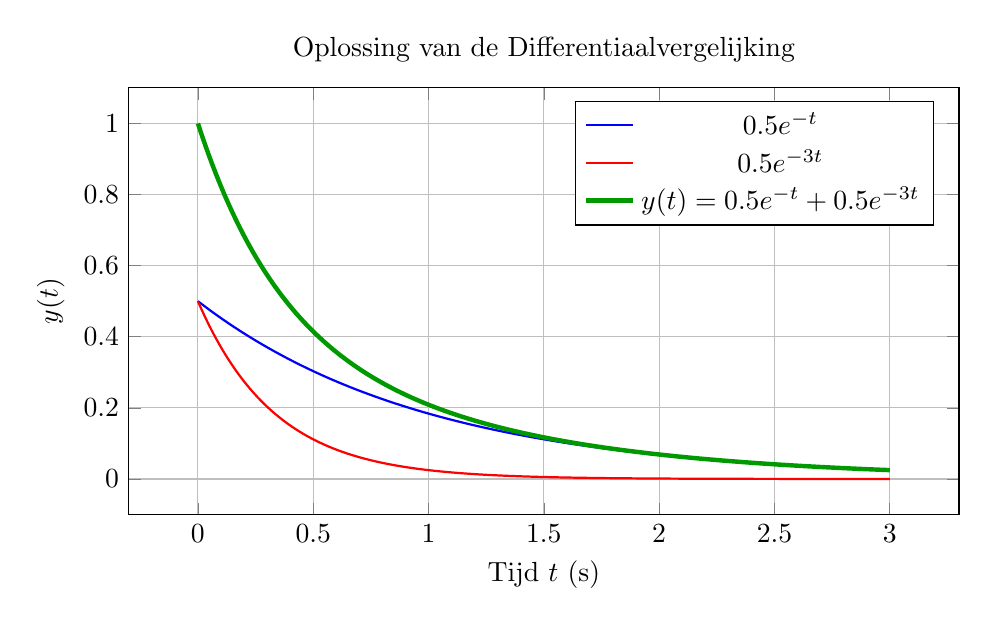
\begin{tikzpicture}
    \begin{axis}[
        width=\textwidth,
        height=7cm,
        xlabel={Tijd \(t\) (s)},
        ylabel={\(y(t)\)},
        title={Oplossing van de Differentiaalvergelijking},
        grid=major,
        legend pos=north east,
        domain=0:3,
        samples=200
    ]
    \addplot[blue, thick] {0.5*exp(-x)};
    \addlegendentry{\(0.5e^{-t}\)}
    
    \addplot[red, thick] {0.5*exp(-3*x)};
    \addlegendentry{\(0.5e^{-3t}\)}
    
    \addplot[green!60!black, ultra thick] {0.5*exp(-x) + 0.5*exp(-3*x)};
    \addlegendentry{\(y(t) = 0.5e^{-t} + 0.5e^{-3t}\)}
    \end{axis}
\end{tikzpicture}
\caption{De oplossing bestaat uit twee exponentieel uitdovende componenten. De snelle component (\(e^{-3t}\)) dempt snel uit, de trage component (\(e^{-t}\)) domineert voor grotere \(t\).}
\end{figure}

\subsection{Oefening 3.3: Begin- en Eindwaardestelling}

\textbf{Gegeven:}
\[
F(s) = \frac{2s + 5}{s^2 + 3s}
\]

\textbf{Vraag:} Bepaal \(f(0^+)\) en \(f(\infty)\) zonder de inverse transformatie te berekenen. Controleer de geldigheid.

\begin{oplossingbox}[Oplossing]

\textbf{Beginwaardestelling:}
\[
f(0^+) = \lim_{s \to \infty} s F(s)
\]

\[
\lim_{s \to \infty} s \frac{2s + 5}{s^2 + 3s} = \lim_{s \to \infty} \frac{2s^2 + 5s}{s^2 + 3s} = \lim_{s \to \infty} \frac{2 + 5/s}{1 + 3/s} = \boxed{2}
\]

\vspace{0.5cm}
\textbf{Eindwaardestelling:}
\[
f(\infty) = \lim_{s \to 0} s F(s)
\]

\textbf{Voorwaarde:} De polen van \(sF(s)\) moeten in het linkerhalfvlak liggen (stabiel).

\[
s F(s) = \frac{s(2s+5)}{s(s+3)} = \frac{2s+5}{s+3}
\]

De pool ligt op \(-3\), dus stabiel. De stelling mag worden toegepast.
\[
\lim_{s \to 0} \frac{2s+5}{s+3} = \frac{5}{3} \approx \boxed{1.667}
\]

\textbf{Conclusie:} De signaalwaarde start op 2 en convergeert naar \(5/3\).
\end{oplossingbox}

% ============================================================================
% HOOFDSTUK 4: FOURIER TRANSFORMATIE
% ============================================================================

\newpage
\section{De Fouriertransformatie}

\begin{theoriebox}[Theoretische Context]
De Fouriertransformatie (FT) ontleedt een signaal in zijn frequentiecomponenten. In tegenstelling tot de Laplace-variabele \(s\) die demping (\(\sigma\)) bevat, focust Fourier puur op oscillatie (\(j\omega\)). 

Dit is essentieel voor het begrijpen van \concept{filtering}, \concept{modulatie} en \concept{signaalbandbreedte}.

\vspace{0.3cm}
\textbf{Belangrijk concept:} \textbf{Dualiteit tussen tijd en frequentie}
\begin{itemize}
    \item Een smalle puls in de tijd resulteert in een breed spectrum
    \item Een breed signaal in de tijd resulteert in een smal spectrum
    \item \(\Delta t \cdot \Delta \omega \geq \text{constante}\) (Onzekerheidsrelatie)
\end{itemize}
\end{theoriebox}

\subsection{Oefening 4.1: Spectrum van een Driehoekpuls}

\textbf{Bepaal de Fouriertransformatie van de driehoekpuls \(\Lambda(t)\) gedefinieerd als:}
\[
\Lambda(t) = \begin{cases}
1 - |t| & \text{voor } |t| < 1 \\
0 & \text{elders}
\end{cases}
\]

\textbf{Tip:} Gebruik het feit dat een driehoek de convolutie is van twee rechthoeken.

\begin{oplossingbox}[Oplossing via Convolutie-eigenschap]

We weten dat de convolutie van twee identieke rechthoekpulsen (rect) een driehoek oplevert.

Laat \(\Pi(t)\) een rechthoek zijn met breedte 1 en hoogte 1 (van \(-0.5\) tot \(0.5\)).

De convolutie \(\Pi(t) * \Pi(t)\) is een driehoek met basis van \(-1\) tot \(1\) en hoogte 1. Dit is exact \(\Lambda(t)\).

De Fouriertransformatie van een rechthoek \(\Pi(t)\) is een sinc-functie:
\[
\mathcal{F}\{\Pi(t)\} = \text{sinc}\left(\frac{\omega}{2}\right)
\]

waarbij \(\text{sinc}(x) = \frac{\sin(x)}{x}\).

Gebruikmakend van de \concept{convolutiestelling}: convolutie in tijd is vermenigvuldiging in frequentie.
\[
\mathcal{F}\{\Lambda(t)\} = \mathcal{F}\{\Pi(t) * \Pi(t)\} = \mathcal{F}\{\Pi(t)\} \cdot \mathcal{F}\{\Pi(t)\}
\]

\[
\boxed{X(\omega) = \left[ \text{sinc}\left(\frac{\omega}{2}\right) \right]^2}
\]

\textbf{Analyse:}

Het spectrum van een driehoekpuls is reëel en positief (kwadraat van sinc). Het daalt sneller af (\(1/\omega^2\)) dan het spectrum van een rechthoek (\(1/\omega\)). 

Dit illustreert een algemene regel: hoe ``gladder'' het signaal in de tijd (driehoek is continu, rechthoek is discontinu), hoe sneller het spectrum afneemt en hoe minder hoge frequenties het bevat.
\end{oplossingbox}

\begin{figure}[H]
\centering
\begin{subfigure}[b]{0.48\textwidth}
\centering
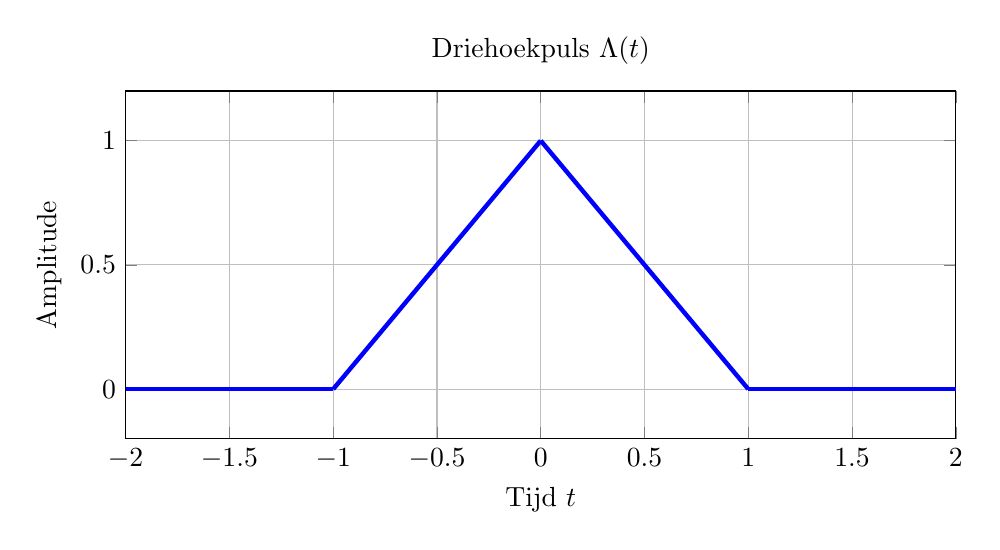
\begin{tikzpicture}
    \begin{axis}[
        width=\textwidth,
        height=6cm,
        xlabel={Tijd \(t\)},
        ylabel={Amplitude},
        title={Driehoekpuls \(\Lambda(t)\)},
        grid=major,
        xmin=-2, xmax=2,
        ymin=-0.2, ymax=1.2
    ]
    \addplot[blue, ultra thick, domain=-2:-1, samples=2] {0};
    \addplot[blue, ultra thick, domain=-1:0, samples=50] {1+x};
    \addplot[blue, ultra thick, domain=0:1, samples=50] {1-x};
    \addplot[blue, ultra thick, domain=1:2, samples=2] {0};
    \end{axis}
\end{tikzpicture}
\caption{Tijdsdomein}
\end{subfigure}
\hfill
\begin{subfigure}[b]{0.48\textwidth}
\centering
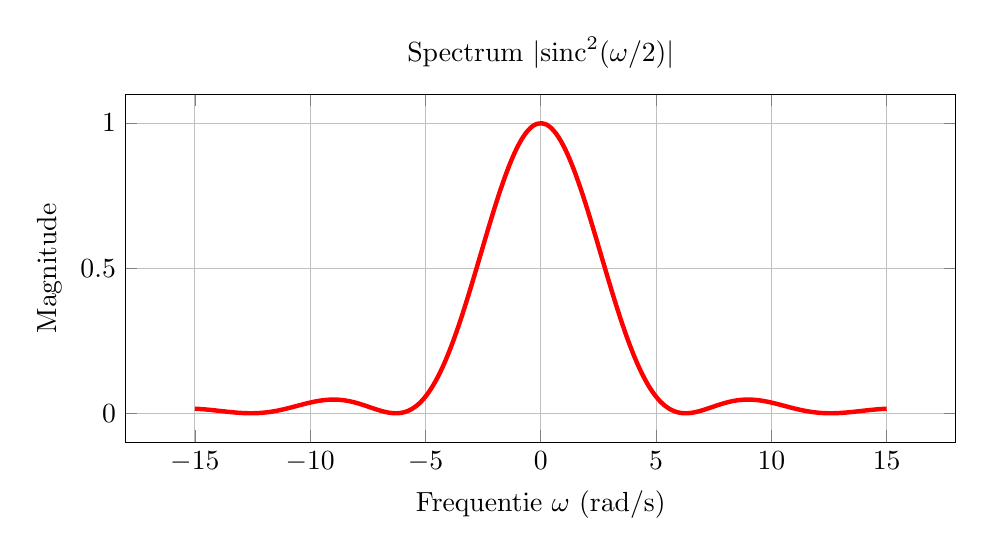
\begin{tikzpicture}
    \begin{axis}[
        width=\textwidth,
        height=6cm,
        xlabel={Frequentie \(\omega\) (rad/s)},
        ylabel={Magnitude},
        title={Spectrum \(|\text{sinc}^2(\omega/2)|\)},
        grid=major,
        domain=-15:15,
        samples=300
    ]
    \addplot[red, ultra thick] {(sin(deg(x/2))/(x/2))^2};
    \end{axis}
\end{tikzpicture}
\caption{Frequentiedomein}
\end{subfigure}
\caption{Driehoekpuls en zijn spectrum. Het spectrum daalt als \(1/\omega^2\), sneller dan bij een rechthoek (\(1/\omega\)).}
\end{figure}

\subsection{Oefening 4.2: Dualiteit en Frequentieverschuiving}

\textbf{Gegeven is dat:}
\[
\mathcal{F}\{e^{-|t|}\} = \frac{2}{1+\omega^2}
\]

\textbf{Vraag:} Bepaal zonder integratie de Fouriertransformatie van het signaal \(x(t) = \frac{1}{1+t^2}\).

\begin{oplossingbox}[Oplossing]

We gebruiken de \concept{dualiteitseigenschap}:

Als \(\mathcal{F}\{f(t)\} = F(\omega)\), dan \(\mathcal{F}\{F(t)\} = 2\pi f(-\omega)\).

In dit geval is de functie \(F(\omega)\) uit het gegeven paar gelijk qua vorm aan onze \(x(t)\).

Stel \(g(t) = e^{-|t|}\), dan \(G(\omega) = \frac{2}{1+\omega^2}\).

We zoeken de transformatie van een functie die lijkt op \(G(t)\).

Laten we \(h(t) = \frac{2}{1+t^2}\). Volgens dualiteit is:
\[
\mathcal{F}\{h(t)\} = 2\pi g(-\omega) = 2\pi e^{-|-\omega|} = 2\pi e^{-|\omega|}
\]

Onze gevraagde functie is \(x(t) = \frac{1}{2} h(t)\). Vanwege lineariteit geldt:
\[
\boxed{\mathcal{F}\{x(t)\} = \frac{1}{2} \mathcal{F}\{h(t)\} = \frac{1}{2} (2\pi e^{-|\omega|}) = \pi e^{-|\omega|}}
\]

\textbf{Resultaat:} Het spectrum van een Lorentz-curve in de tijd is een dubbele exponentiaal in het frequentiedomein. Dit is een mooi voorbeeld van de symmetrie tussen tijd- en frequentiedomein.
\end{oplossingbox}

\begin{figure}[H]
\centering
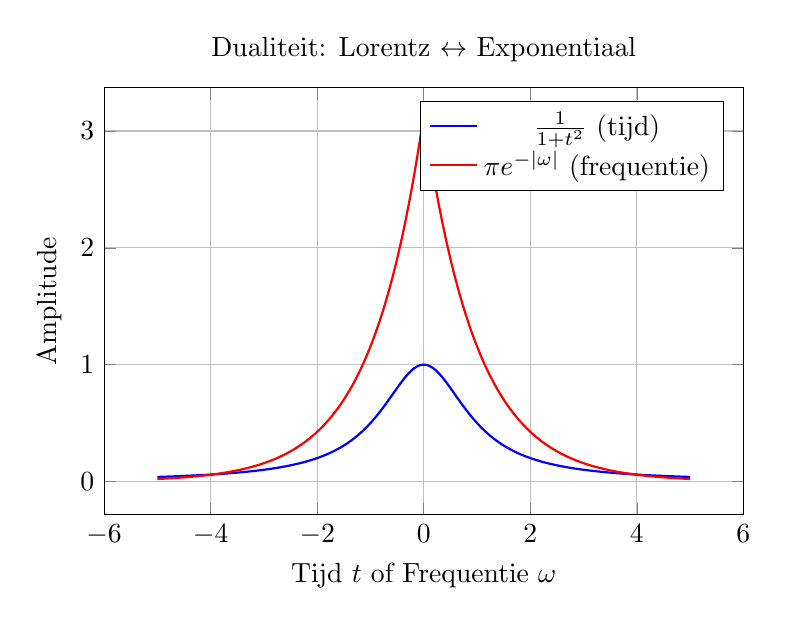
\begin{tikzpicture}
    \begin{axis}[
        width=0.8\textwidth,
        height=7cm,
        xlabel={Tijd \(t\) of Frequentie \(\omega\)},
        ylabel={Amplitude},
        title={Dualiteit: Lorentz \(\leftrightarrow\) Exponentiaal},
        grid=major,
        legend pos=north east,
        domain=-5:5,
        samples=200
    ]
    \addplot[blue, thick] {1/(1+x^2)};
    \addlegendentry{\(\frac{1}{1+t^2}\) (tijd)}
    
    \addplot[red, thick] {pi*exp(-abs(x))};
    \addlegendentry{\(\pi e^{-|\omega|}\) (frequentie)}
    \end{axis}
\end{tikzpicture}
\caption{De Lorentz-curve in tijdsdomein correspondeert met een exponentieel spectrum. Dit is een perfect symmetrisch transformatiepaar.}
\end{figure}

% ============================================================================
% VERVOLG IN DEEL 2 VANWEGE LENGTE
% ============================================================================

\newpage
\section{De Fourierreeks}

\begin{theoriebox}[Theoretische Context]
Voor \textbf{periodieke} signalen is het spectrum niet continu, maar \textbf{discreet}. Het signaal bevat enkel frequenties die veelvouden zijn van de grondfrequentie \(\omega_0 = 2\pi/T\).

De Fourierreeks drukt het signaal uit als een som van deze harmonischen:
\[
x(t) = \sum_{k=-\infty}^{\infty} c_k e^{jk\omega_0 t}
\]

waarbij de complexe coëfficiënten:
\[
c_k = \frac{1}{T} \int_0^T x(t) e^{-jk\omega_0 t} \, dt
\]

\textbf{Symmetrie-eigenschappen} kunnen het werk aanzienlijk vereenvoudigen:
\begin{itemize}
    \item Even signaal: enkel cosinus-termen (reële coëfficiënten)
    \item Oneven signaal: enkel sinus-termen (imaginaire coëfficiënten)
\end{itemize}
\end{theoriebox}

\subsection{Oefening 5.1: Fourierreeks van een Gelijkgerichte Sinus}

\textbf{Beschouw het signaal:}
\[
x(t) = |\sin(t)|
\]

\textbf{Vragen:}
\begin{enumerate}
    \item Wat is de fundamentele periode \(T\)?
    \item Bepaal de complexe Fouriercoëfficiënten \(c_k\).
\end{enumerate}

\begin{oplossingbox}[Oplossing]

\textbf{1. Periode}

Hoewel \(\sin(t)\) periode \(2\pi\) heeft, zorgt de absolute waarde ervoor dat het negatieve deel wordt omgeklapt. De vorm herhaalt zich dus elke \(\pi\).

\(T = \pi\). Grondfrequentie \(\omega_0 = \frac{2\pi}{T} = \frac{2\pi}{\pi} = 2\) rad/s.

\vspace{0.5cm}
\textbf{2. Coëfficiënten}

Formule: \(c_k = \frac{1}{T} \int_0^T x(t) e^{-jk\omega_0 t} \, dt\).
\[
c_k = \frac{1}{\pi} \int_0^{\pi} \sin(t) e^{-j2kt} \, dt
\]

Gebruik de Euler-vorm voor sinus: \(\sin(t) = \frac{e^{jt} - e^{-jt}}{2j}\).
\[
c_k = \frac{1}{2j\pi} \int_0^{\pi} (e^{jt} - e^{-jt}) e^{-j2kt} \, dt
\]

\[
c_k = \frac{1}{2j\pi} \int_0^{\pi} (e^{j(1-2k)t} - e^{-j(1+2k)t}) \, dt
\]

Los de integraal op:
\[
\int_0^{\pi} e^{j(1-2k)t} \, dt = \left[ \frac{e^{j(1-2k)t}}{j(1-2k)} \right]_0^{\pi} = \frac{e^{j\pi} e^{-j2k\pi} - 1}{j(1-2k)}
\]

We weten dat \(e^{-j2k\pi} = 1\) (want \(k\) is integer) en \(e^{j\pi} = -1\). Dus de teller is \(-1 - 1 = -2\).

Eerste term: \(\frac{-2}{j(1-2k)}\).

De tweede term wordt analoog \(\frac{-2}{-j(1+2k)} = \frac{2}{j(1+2k)}\).

Combineren:
\begin{align*}
c_k &= \frac{1}{2j\pi} \left( \frac{-2}{j(1-2k)} - \frac{2}{j(1+2k)} \right) \\
&= \frac{1}{2j\pi} \cdot \frac{1}{j} \left( \frac{-2}{1-2k} - \frac{2}{1+2k} \right) \\
&= \frac{-1}{2\pi} \left( \frac{-2(1+2k) - 2(1-2k)}{(1-2k)(1+2k)} \right) \\
&= \frac{-1}{2\pi} \left( \frac{-4}{1 - 4k^2} \right)
\end{align*}

\[
\boxed{c_k = \frac{2}{\pi(1 - 4k^2)}}
\]

\textbf{Resultaat:} De coëfficiënten zijn reëel en afnemen als \(1/k^2\). Dit komt omdat het signaal even is en geen discontinuïteiten heeft (wel knikpunten).
\end{oplossingbox}

\begin{figure}[H]
\centering
\begin{subfigure}[b]{0.48\textwidth}
\centering
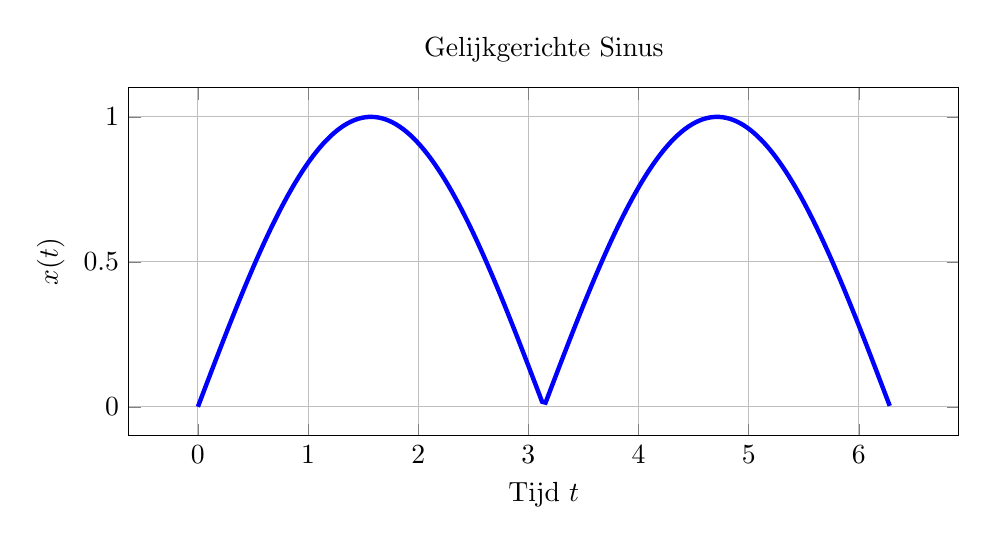
\begin{tikzpicture}
    \begin{axis}[
        width=\textwidth,
        height=6cm,
        xlabel={Tijd \(t\)},
        ylabel={\(x(t)\)},
        title={Gelijkgerichte Sinus},
        grid=major,
        domain=0:6.28,
        samples=200
    ]
    \addplot[blue, ultra thick] {abs(sin(deg(x)))};
    \end{axis}
\end{tikzpicture}
\caption{Tijdsdomein: Periode \(T = \pi\)}
\end{subfigure}
\hfill
\begin{subfigure}[b]{0.48\textwidth}
\centering
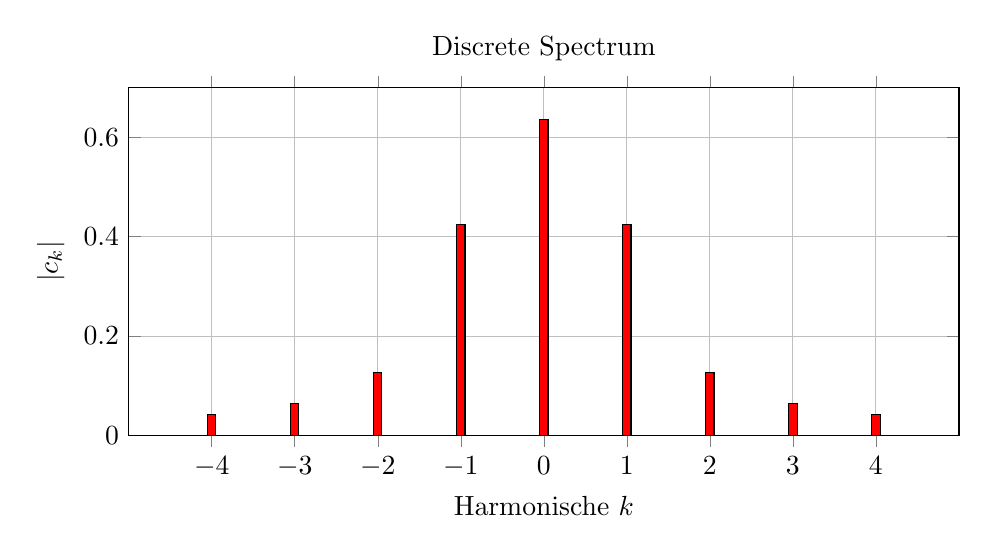
\begin{tikzpicture}
    \begin{axis}[
        width=\textwidth,
        height=6cm,
        xlabel={Harmonische \(k\)},
        ylabel={\(|c_k|\)},
        title={Discrete Spectrum},
        ybar,
        bar width=3pt,
        grid=major,
        xmin=-5, xmax=5,
        ymin=0, ymax=0.7,
        xtick={-4,-3,-2,-1,0,1,2,3,4}
    ]
    \addplot[fill=red] coordinates {
        (-4, 0.0424)
        (-3, 0.0637)
        (-2, 0.1273)
        (-1, 0.4244)
        (0, 0.6366)
        (1, 0.4244)
        (2, 0.1273)
        (3, 0.0637)
        (4, 0.0424)
    };
    \end{axis}
\end{tikzpicture}
\caption{Frequentiedomein: Discrete lijnen}
\end{subfigure}
\caption{Gelijkgerichte sinus en zijn discrete frequentiespectrum. De coëfficiënten nemen snel af (\(1/k^2\)).}
\end{figure}

% ============================================================================
% HOOFDSTUK 6: LTI-SYSTEMEN
% ============================================================================

\newpage
\section{LTI-Systemen en Frequentierespons}

\begin{theoriebox}[Theoretische Context]
LTI-systemen worden gekenmerkt door hun \concept{transferfunctie} \(H(s)\), wat de verhouding is tussen de Laplacetransformatie van de output en de input:
\[
H(s) = \frac{Y(s)}{X(s)}
\]

De \concept{frequentierespons} \(H(j\omega)\) beschrijft hoe het systeem reageert op sinusoïdale inputs. 

\textbf{Cruciale eigenschap:} Een LTI-systeem verandert de frequentie van een sinusoïde niet, maar enkel:
\begin{itemize}
    \item De amplitude (vermenigvuldiging met \(|H(j\omega)|\))
    \item De fase (optelling met \(\angle H(j\omega)\))
\end{itemize}
\end{theoriebox}

\subsection{Oefening 6.1: Respons op een Sinus}

\textbf{Een systeem heeft een transferfunctie:}
\[
H(s) = \frac{10}{s + 2}
\]

\textbf{Vraag:} Bepaal de steady-state output \(y_{ss}(t)\) als de input \(x(t) = 3 \cos(2t + 45^\circ)\) is.

\begin{oplossingbox}[Oplossing]

\textbf{1. Frequentierespons bepalen}

Vervang \(s\) door \(j\omega\). De inputfrequentie is \(\omega = 2\) rad/s.
\[
H(j2) = \frac{10}{j2 + 2} = \frac{10}{2 + 2j} = \frac{10}{2(1+j)}
\]

\vspace{0.3cm}
\textbf{2. Magnitude en Fase berekenen}

Magnitude:
\[
|H(j2)| = \frac{|10|}{|2+2j|} = \frac{10}{\sqrt{2^2 + 2^2}} = \frac{10}{2\sqrt{2}} = \frac{5}{\sqrt{2}} \approx 3.536
\]

Fase:
\[
\angle H(j2) = \angle 10 - \angle (2+2j) = 0^\circ - \arctan\left(\frac{2}{2}\right) = 0^\circ - 45^\circ = -45^\circ
\]

\vspace{0.3cm}
\textbf{3. Output samenstellen}

De output amplitude is:
\[
A_{\text{out}} = A_{\text{in}} \times |H(j\omega)| = 3 \times 3.536 = 10.61
\]

De output fase is:
\[
\phi_{\text{out}} = \phi_{\text{in}} + \angle H(j\omega) = 45^\circ - 45^\circ = 0^\circ
\]

\[
\boxed{y_{ss}(t) = 10.61 \cos(2t)}
\]

\textbf{Interpretatie:} Het systeem versterkt het signaal en introduceert een fasevertraging die de oorspronkelijke fase toevallig precies annuleert. Dit is een voorbeeld van een laagdoorlaatfilter (pool bij \(s=-2\)).
\end{oplossingbox}

\begin{figure}[H]
\centering
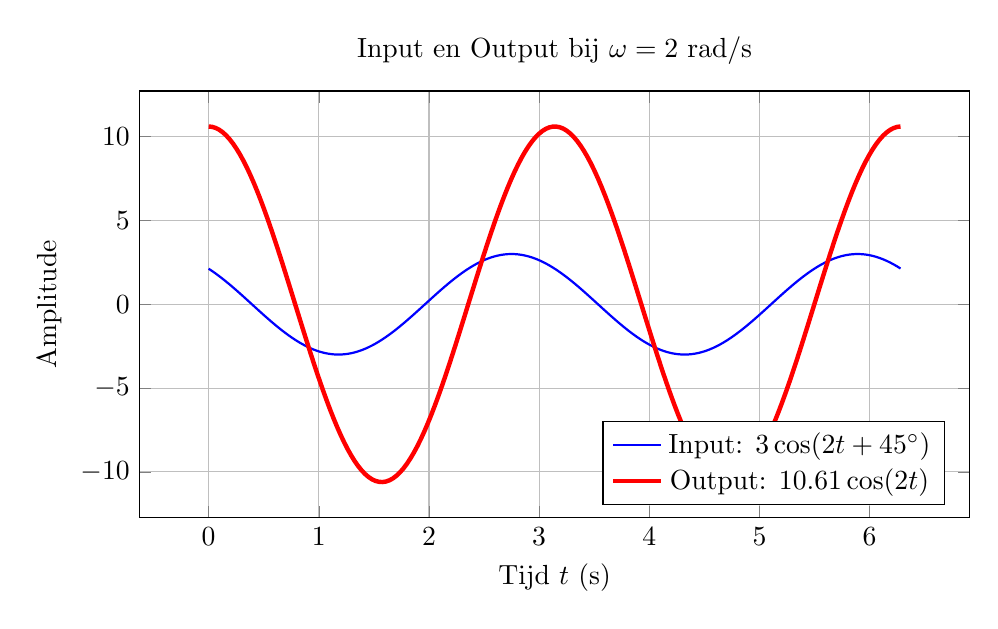
\begin{tikzpicture}
    \begin{axis}[
        width=\textwidth,
        height=7cm,
        xlabel={Tijd \(t\) (s)},
        ylabel={Amplitude},
        title={Input en Output bij \(\omega = 2\) rad/s},
        grid=major,
        legend pos=south east,
        domain=0:6.28,
        samples=200
    ]
    \addplot[blue, thick] {3*cos(deg(2*x + 0.7854))};
    \addlegendentry{Input: \(3\cos(2t + 45^\circ)\)}
    
    \addplot[red, ultra thick] {10.61*cos(deg(2*x))};
    \addlegendentry{Output: \(10.61\cos(2t)\)}
    \end{axis}
\end{tikzpicture}
\caption{Het systeem versterkt de amplitude en verschuift de fase met \(-45^\circ\), wat de oorspronkelijke \(+45^\circ\) precies compenseert.}
\end{figure}

\subsection{Oefening 6.2: Stabiliteitsanalyse via Polen}

\textbf{Bepaal voor welke waarden van \(K\) het teruggekoppelde systeem met open-lus transferfunctie stabiel is:}
\[
G(s) = \frac{K}{s(s+1)(s+2)}
\]

\begin{oplossingbox}[Oplossing]

De gesloten-lus transferfunctie is \(T(s) = \frac{G(s)}{1 + G(s)}\).

De polen worden bepaald door de karakteristieke vergelijking \(1 + G(s) = 0\):
\[
1 + \frac{K}{s(s+1)(s+2)} = 0 \implies s(s+1)(s+2) + K = 0
\]

\[
s(s^2 + 3s + 2) + K = s^3 + 3s^2 + 2s + K = 0
\]

\textbf{Gebruik het Routh-Hurwitz criterium:}

Opstellen van de Routh-tabel:
\begin{center}
\begin{tabular}{c|cc}
\(s^3\) & 1 & 2 \\
\(s^2\) & 3 & K \\
\(s^1\) & \(\frac{3(2) - 1(K)}{3} = \frac{6-K}{3}\) & 0 \\
\(s^0\) & K &
\end{tabular}
\end{center}

Voor stabiliteit moeten alle elementen in de eerste kolom \textbf{positief} zijn:
\begin{enumerate}
    \item \(3 > 0\) \checkmark (altijd OK)
    \item \(\frac{6-K}{3} > 0 \implies 6 > K\)
    \item \(K > 0\)
\end{enumerate}

\[
\boxed{0 < K < 6}
\]

\textbf{Conclusie:} Het systeem is stabiel voor \(0 < K < 6\). Bij \(K=6\) zal het systeem oscilleren (marginaal stabiel), en bij \(K>6\) wordt het onstabiel (polen in het rechterhalfvlak).
\end{oplossingbox}

\begin{figure}[H]
\centering
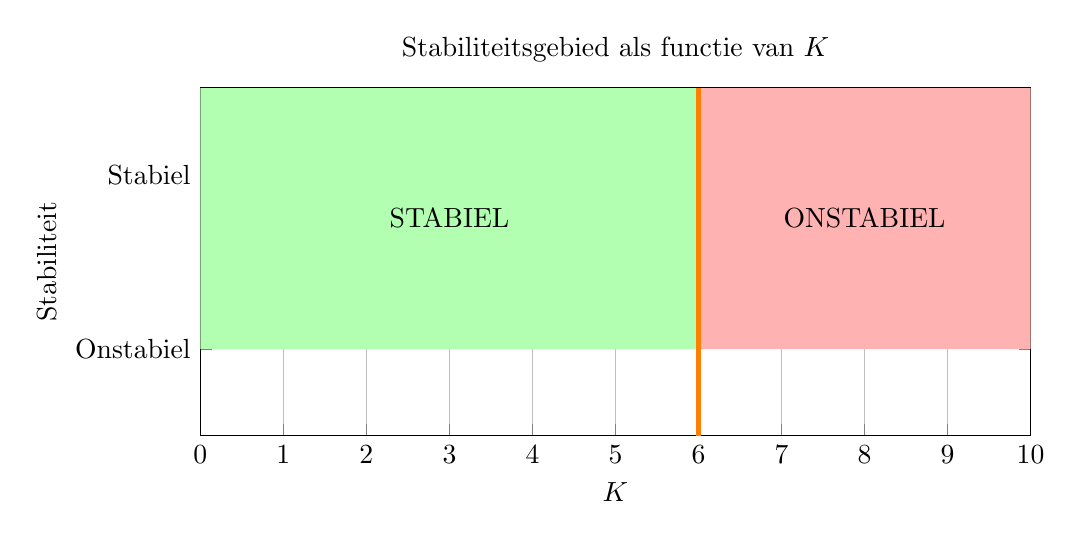
\begin{tikzpicture}
    \begin{axis}[
        width=\textwidth,
        height=6cm,
        xlabel={\(K\)},
        ylabel={Stabiliteit},
        title={Stabiliteitsgebied als functie van \(K\)},
        xmin=0, xmax=10,
        ymin=0, ymax=2,
        ytick={0.5, 1.5},
        yticklabels={Onstabiel, Stabiel},
        grid=major
    ]
    % Stabiel gebied
    \fill[green!30] (axis cs:0,0.5) rectangle (axis cs:6,2);
    \node at (axis cs:3,1.25) {STABIEL};
    
    % Onstabiel gebied
    \fill[red!30] (axis cs:6,0.5) rectangle (axis cs:10,2);
    \node at (axis cs:8,1.25) {ONSTABIEL};
    
    % Kritieke waarde
    \draw[ultra thick, orange] (axis cs:6,0) -- (axis cs:6,2);
    \node[above, orange] at (axis cs:6,2) {\(K=6\)};
    \end{axis}
\end{tikzpicture}
\caption{Stabiliteitsanalyse: Het systeem is stabiel voor \(0 < K < 6\). Bij \(K=6\) treedt marginale stabiliteit op.}
\end{figure}

% ============================================================================
% SAMENVATTING EN FORMULES
% ============================================================================

\newpage
\section*{Appendix: Belangrijke Formules en Transformatieparen}

\subsection*{Laplace-Transformatieparen}

\begin{center}
\begin{tabular}{|c|c|c|}
\hline
\textbf{Signaal \(x(t)\)} & \textbf{Laplace \(X(s)\)} & \textbf{ROC} \\
\hline
\(\delta(t)\) & \(1\) & Alle \(s\) \\
\(u(t)\) & \(\frac{1}{s}\) & \(\text{Re}(s) > 0\) \\
\(t \cdot u(t)\) & \(\frac{1}{s^2}\) & \(\text{Re}(s) > 0\) \\
\(e^{-at}u(t)\) & \(\frac{1}{s+a}\) & \(\text{Re}(s) > -a\) \\
\(t e^{-at}u(t)\) & \(\frac{1}{(s+a)^2}\) & \(\text{Re}(s) > -a\) \\
\(\cos(\omega_0 t) u(t)\) & \(\frac{s}{s^2 + \omega_0^2}\) & \(\text{Re}(s) > 0\) \\
\(\sin(\omega_0 t) u(t)\) & \(\frac{\omega_0}{s^2 + \omega_0^2}\) & \(\text{Re}(s) > 0\) \\
\(e^{-at}\cos(\omega_0 t) u(t)\) & \(\frac{s+a}{(s+a)^2 + \omega_0^2}\) & \(\text{Re}(s) > -a\) \\
\(e^{-at}\sin(\omega_0 t) u(t)\) & \(\frac{\omega_0}{(s+a)^2 + \omega_0^2}\) & \(\text{Re}(s) > -a\) \\
\hline
\end{tabular}
\end{center}

\subsection*{Fourier-Transformatieparen}

\begin{center}
\begin{tabular}{|c|c|}
\hline
\textbf{Signaal \(x(t)\)} & \textbf{Fourier \(X(j\omega)\)} \\
\hline
\(\delta(t)\) & \(1\) \\
\(1\) & \(2\pi\delta(\omega)\) \\
\(\text{sinc}(t)\) & \(\text{rect}(\omega / 2\pi)\) \\
\(e^{-|t|}\) & \(\frac{2}{1 + \omega^2}\) \\
\(\cos(\omega_0 t)\) & \(\pi[\delta(\omega-\omega_0) + \delta(\omega+\omega_0)]\) \\
\(e^{-at}u(t)\), \(a>0\) & \(\frac{1}{a + j\omega}\) \\
\hline
\end{tabular}
\end{center}

\subsection*{Eigenschappen}

\begin{center}
\begin{tabular}{|l|c|c|}
\hline
\textbf{Eigenschap} & \textbf{Tijd} & \textbf{Frequentie (Laplace)} \\
\hline
Lineariteit & \(\alpha x_1(t) + \beta x_2(t)\) & \(\alpha X_1(s) + \beta X_2(s)\) \\
Tijdsverschuiving & \(x(t-t_0)\) & \(e^{-st_0}X(s)\) \\
Frequentieverschuiving & \(e^{s_0 t}x(t)\) & \(X(s-s_0)\) \\
Schaling & \(x(at)\) & \(\frac{1}{|a|}X(s/a)\) \\
Convolutie & \(x(t) * h(t)\) & \(X(s) \cdot H(s)\) \\
Differentiatie & \(\frac{dx(t)}{dt}\) & \(sX(s) - x(0^-)\) \\
Integratie & \(\int_{-\infty}^{t} x(\tau) d\tau\) & \(\frac{X(s)}{s}\) \\
\hline
\end{tabular}
\end{center}

\subsection*{Stabiliteit}

\begin{tcolorbox}[title=Stabiliteitsregels, colback=blue!5, colframe=blue!75!black]
Een systeem is \textbf{BIBO stabiel} als en slechts als:
\begin{enumerate}
    \item Alle polen van \(H(s)\) liggen in het open linkerhalfvlak: \(\text{Re}(s) < 0\)
    \item Of equivalent: \(\int_{-\infty}^{\infty} |h(t)| \, dt < \infty\)
\end{enumerate}

\textbf{Marginaal stabiel:} Polen op de imaginaire as (geen herhaalde polen).

\textbf{Onstabiel:} Minstens één pool in het rechterhalfvlak: \(\text{Re}(s) > 0\).
\end{tcolorbox}

\end{document}